\documentclass{sig-alternate}

\usepackage[utf8]{inputenc}
\usepackage{natbib}

%\usepackage[utf8]{inputenc}
%\usepackage[backend = bibtex, citestyle=authoryear]{biblatex}

%\usepackage[american]{babel}
%\usepackage{csquotes}
%\usepackage[style=apa]{biblatex}
%\DeclareLanguageMapping{american}{american-apa}

%\addbibresource{library.bib}
%\usepackage{fullpage}

%Math mode

\usepackage{amsmath}
\usepackage{amsfonts}
\usepackage{amssymb}
%\usepackage{amsthm}
\usepackage{dsfont}
%\usepackage{mathtools}
\usepackage{xfrac}
%\usepackage{thmtools}
\usepackage{bm}

% CODE

\usepackage{courier}

\usepackage{listings}
\usepackage{color} %red, green, blue, yellow, cyan, magenta, black, white
\definecolor{mygreen}{RGB}{28,172,0} % color values Red, Green, Blue
\definecolor{mylilas}{RGB}{170,55,241}
\usepackage{marginnote}
\usepackage[linktocpage, breaklinks, colorlinks = true, linkcolor = Brown, citecolor = blue]{hyperref}
\usepackage{enumerate}

%PS_tricks

\usepackage[usenames,dvipsnames]{pstricks}
\usepackage{epsfig}
\usepackage{pst-grad} % For gradients
\usepackage{pst-plot} % For axes
\usepackage{float}

\usepackage{nameref}
\usepackage{mdframed}
\usepackage{accents}

%Geometry
%\usepackage[lmargin=3.5cm,rmargin=3.5cm,tmargin=2cm,bmargin=2cm,marginpar=3cm]{geometry}

%Proof style

%\renewcommand\qedsymbol{$\blacksquare$}

% %Margin style

\renewcommand*{\marginfont}{\footnotesize}

% %Graphic path

\graphicspath{{graphics/}}

% %Theorem Environments

%\declaretheorem [name = Theorem]{theo}
%\declaretheorem [name = Corollary]{coro}
%\declaretheorem [name = Lemma]{lem}
%\declaretheorem [name = Fairness Axiom]{ax}
%\declaretheorem [name = Preference axiom]{pref}
%\declaretheorem [name = Profile axiom]{prof}
%\declaretheorem [name = Observation]{obs}
%\declaretheorem [name = Definition]{defi}
%\declaretheorem [name = Social ordering function]{sof}
%\declaretheorem [name = Proposition, unnumbered]{prop}
%\declaretheorem [name = Example, unnumbered]{expl}
%
% %In-text hyppereff

\newcommand{\nref}{\nameref}

% %Short commands for math mode

%Style

\newcommand{\mb}[1]{\mathbf{#1}}     % bold letters in mathmode
\newcommand{\bs}[1]{\boldsymbol{#1}} % bold symbols in mathmode
\newcommand{\bb}[1]{\mathbb{#1}}     % Doppelstrichbuchstaben im Mathematikmodus

\newcommand{\mc}[1]{\mathcal{#1}}    % calligraphy style

%Sets

\newcommand{\rr}{\bb{R}} % set of reals in mathmode

%Fractions

\newcommand{\pfraca}[2]{\bigl(\frac{#1}{#2}\bigr)}    % ratios with small parantheses
\newcommand{\pfracb}[2]{\Bigl(\frac{#1}{#2}\Bigr)}    % ratios with big parantheses
\newcommand{\pfracc}[2]{\biggl(\frac{#1}{#2}\biggr)}  % ratios with bigger parantheses
\newcommand{\pfracd}[2]{\Biggl(\frac{#1}{#2}\Biggr)}  % ratios with huge parantheses

%Partial derivatives

\newcommand{\di}[1]{\frac{\partial}{\partial #1}}     % shortcut for first partial derivative
\newcommand{\dii}[1]{\frac{\partial^2}{\partial #1^2}}% shortcut for second partial derivative

%other

\newcommand{\ra}{\rightarrow}            

%Convergence

\newcommand{\cd}{\overset{d}{\rightarrow}}    % convergence in distribution
\newcommand{\cp}{\overset{p}{\rightarrow}}    % convergence in probability
\newcommand{\cas}{\overset{as}{\rightarrow}}  % convergence almost surely

%Text in math environment

\newcommand{\sgn}{~\text{sgn}~}
\newcommand{\f}{~\text{if}~}
\newcommand{\frall}{~\text{for all}~}
\newcommand{\ow}{~\text{otherwise}~}
\newcommand{\nd}{~\text{and}~}
\newcommand{\thn}{~\text{then}~}
\newcommand{\id}{\coloneqq}

%Variant of variables (tilde, lower bar,...)

\newcommand{\lbar}[1]{\underline{#1\mkern-4mu}\mkern4mu }

\newcommand{\x}{\bm{x}}
\newcommand{\m}{\bm{m}}
\newcommand{\z}{\bm{z}}
\newcommand{\g}{\bm{\gamma}}
\newcommand{\h}{\bm{h}}
\newcommand{\y}{\bm{y}}
\newcommand{\e}{\bm{e}}
\newcommand{\la}{\bm{\lambda}}
\newcommand{\ce}{\bm{c}}
\renewcommand{\b}{\bm{\beta}}
\newcommand{\hb}{\hat{\b}}

\clubpenalty=10000
\widowpenalty = 10000 

\usepackage[hyphenbreaks]{breakurl}
%\usepackage[hyphens]{url}
	
\begin{document}

	
	\title{Prediction Markets and Congruence of Predictive Models:
  An Agent-Based Simulation of Climate Prediction Markets}
  %\substitle{An Agent-Based Simulation of Climate Prediction Markets}
	
	\numberofauthors{2} 
	\author{
    \alignauthor
		John J. Nay
		\alignauthor
		Martin Van der Linden
	}
		
	
	\maketitle
	\begin{abstract}
We present an agent-based model (ABM) of a climate prediction market in which traders adapt their belief about the climate based on the monetary performance of their neighboring traders in a social network. We use the ABM to test whether climate prediction markets fosters a convergence of market participants' beliefs regarding a ``true'' climate model. We provide preliminary sensitivity analysis for the impact on the convergence of factors such as the initial belief-homophily in the social network and the degree of risk-taking of traders on the market.
	\end{abstract}
	
	
	\section{Introduction}
	
	The previous two decades saw a strong polarization of the climate change debate. Although the scientific consensus on the anthropogenic nature of climate change strongly increased,  the average belief about anthropogenic climate change did not evolve much within the public (see \cite{Vandenbergh2013f} for all the claims in this paragraph). In addition, the divide on anthropogenic climate change between liberals and conservatives has grown steadily, indicating that the question is becoming more and more politicized and potentially disconnected from scientific evidence.
	
	This is worrisome given the costs of a misinformed climate policy. If anthropocentric climate change is a myth but is taken to be true, a tremendous amount of public resources will be wasted on adaptation and mitigation efforts. On the other hand, if anthropocentric climate change is wrongly consider as false, the costs of inaction would be huge. Given that effective climate policies require long-lasting measures to be taken, the importance of an accurate consensus on the issue is manifest. 
	
	Attempts to foster such consensus face many \linebreak  social and psychological challenges (see \cite[Sections II.B to II.D]{Vandenbergh2013f} for a review). Recently, people have argued that such challenges could be met by setting up climate prediction markets (see for instance \cite{Hsu2011}, and \cite{Vandenbergh2013f}). The idea of using prediction markets to efficiently aggregate information about uncertain events has been discussed for decades (see \cite{Horn2014c} for a recent review). Prediction markets have been shown to have interesting theoretical properties (e.g. \cite{Set1998}, \cite{Hanson2012}, ) and to perform well in terms of prediction accuracy in experiments (e.g \cite{Hanson2006}, \cite{Healy2010}), agent-based models (henceforth ABM) ( e.g \cite{Klingert2012c}, \cite{Jumadinova2011a}), and in the real-world (see \cite{Wolfers2006} for a review).
	
However, to the best of our knowledge, the idea that prediction markets can generate a consensus \emph{on the factors} affecting  uncertain events has never been quantitatively tested. ABMs of prediction markets have been studied ( e.g. \cite{Klingert2012c}, \cite{Tseng2010a}, or\cite{Jumadinova2011a}), some of which feature communication between agents. In these models, however, beliefs about the uncertain outcomes are constructed in rather abstract ways. In particular, beliefs are never based on structural models from which agents would derive causal implications. Therefore, although convergence of beliefs could be studied in previous ABMs, these models do not investigate the convergence of the underlying explanatory models agents use for prediction (more details in section \ref{related}).

From a public policy perspective, this is a crucial point. Effective climate policy not only requires an accurate consensus on future climate \emph{outcomes}. It also requires an accurate consensus on the causal \emph{mechanisms}  influencing such outcomes. If people agree that temperature will rise, but some believe it will be due to greenhouse gases, while others believe that it will be caused by increased solar activity, inconsistent and ineffective policy will may be implemented. In this project, we investigate whether prediction markets can foster such convergence in predictive models.

The main questions we want to answer are:

\begin{enumerate}
	\item Do traders' predictive models converge to the true model, or can traders converge to a ``bad" equilibrium in which most people believe in a wrong predictive model?
	\item How is convergence to the true model affected by the parameters and assumptions of the model such as:
	\begin{enumerate}
		 \item The initial homophily of the network. A strongly homophil network has traders connect preferably with other traders having the same beliefs. Given the political polarization of beliefs in climate change, this homophily is likely to be a feature of a climate change belief network. One may therefore wonder under which conditions of initial homophily could prediction market decluster the belief networks.
		 \item The timing of the market. \cite{Vandenbergh2013f} have argued that prediction market should trade securities based on long term outcomes in order to guarantee that the market provides information about climate rather than weather. However, long term trading might slow down convergence. For a trader $i$ to change her predictive model and adopt the model of another trader $j$, $i$ must be convinced  that $j$'s model is better. If $i$ relies on the market performances of $j$ to evaluate $j$'s models, $i$ will have to wait that securities be realized before she adapt their explanatory model. If the securities are based on long term outcomes, then traders will not adapt their model for before a while. Therefore, there may be a trade-off between speed and accuracy. 
		 \item The model assumed to be the true model of the climate. An important argument in favor of a climate prediction market is that it is supposed to be an apartisan proposal. Defenders of climate prediction markets argue that climate prediction markets will foster convergence to the best approximate model, whatever the actual true model is. If climate change is not anthropogenic -- so the argument goes, traders will converge to non-anthropogenic in pretty much the same way as they would converge to anthropogenic models if the climate is truly influenced by human activities. 
	\end{enumerate}
\end{enumerate}

In this report, we provide preliminary results regarding question 1 and 2.a), together with sensitivity analyses for other parameters of the model. See section \ref{results} for important caveats regarding these results. Despite these caveats, our first exploratory investigation raise a couple of interesting questions. 

First, we observe that convergence to the true model is by no means inevitable. In the model, traders adapt their beliefs based on their neighbors monetary performance on the market (more in Section \ref{implem}). Therefore, one might expect that traders with the right model of the climate will perform better and  convince their (social network) neighbors to believe in the true model. We find that this is not always the case. On \url{https://www.youtube.com/watch?v=MS4YfhTU-WY}, one can see the evolution of the belief network for some particular values of the parameter. In this case, the green and red nodes correspond to traders believeing in predictive models which are qualitatively very far from the true model (see below). One sees that these models are progressively eliminated from the network. On \url{https://www.youtube.com/watch?v=aDB7UY7bDGE} however, initial homophily is increased and the network is sufficiently clustered at the outset to prevent convergence. In Section \ref{results} we provide further evidence on the possibility of non-convergence.  The reason of such non-convergence and the precise conditions on parameters which favor convergence are an open question that we plan to tackle in the near future. 


% So far, we have been able to construct a minimal model of a prediction market. In  the model, traders update their explanatory model of the climate based on the model of their neighbors in a social network. If a trader believe in model $x$ and is surrounded by traders believing in model $y$ who happen to do much better then her on the market, then there is a probability that $x$ will change her explanatory model for the model of trader $x$. 
% 
% At this point the model is not complete. In particular, it features a single market mechanism known as the continuous double auction ( CDA). We plan on implementing at least a second market mechanism known as the logarithmic market scoring rule (LMSR, \cite{Hanson2012}) in order to compare the performance of both mechanism in terms of prediction accuracy and explanatory model convergence. We also need to work on relating some of the parameters with the theoretical literature on network analysis and decision making.\footnote{For instance, we have a parameter which influence the initial level of clustering in the network. We need to work on relating the value of this coefficient with commonly used clustering measures in the network literature.} 

  \section{Related Work}
	\label{related}
	
	\cite{Tseng2010a} study an ABM of a continuous double auction model with various types of market strategies (including two variants of the zero-intelligence agents). They compare the behavior of their simulation with data from a prediction market for the outcome of political elections. They find that despite their simplicity, zero-intelligence agents capture some salient features of real market data. \cite{Klingert2012c} reach similar conclusions with respect to experimental data from  \cite{Hanson2006}. In their simulation, \cite{Klingert2012c} compare continuous double auctions with logarithmic market scoring rules and find that the latter generally outperform continuous double auctions in terms of prediction accuracy. In some variants of the two last models, agents' strategies feature learning, but these are rather basic and unrelated to a formal predictive model. 
	
	\cite{Jumadinova2011a} conducted research more similar to our project, as they explicitly include information about uncertain events in their model. The paper studies a continuous double auction model in which agents update their beliefs about the uncertain events based on information on the event. New beliefs are modeled as a weighted sum of the last period's beliefs and market prices. The agent's information set changes every period. The better the information set, the more likely the agent is to put higher weights on last period's prices when revising their beliefs. Not much structure is imposed on the information set and the way it is used to generate the weights in the update function. Therefore, the model does not allow for investigating the convergence of predictive models. \cite{Ontanon2009} study the effect of deliberation on a simulated prediction market. They assume that agents use Case-Based Reasoning \citep{Aamodt1994} to debate about  uncertain outcomes with their neighbors in a social network.  Although the model could in theory be used to assess convergence of predictive models by looking at the arguments agents adopt after the deliberation, this is not done by the authors. Also, the way beliefs are formed and revised through argumentation is rather abstract and might not be ideal to study climate prediction markets.
 
	
	\section{Model}
	
	\label{model}
	
	In its current form, the ABM is composed of the following elements.
	
	\begin{description}
		\setlength\itemsep{0em}
		\item [A simple ``true" model $F$ of world temperatures.] The model is an additive autoregressive function and is taken  from \cite{Sumner2008b} (it is a simplified version of  RICE99 from \cite{Nordhaus}).
		\begin{align}
		\label{true}
		\begin{split}
				T_t ~ =~  \lambda T_{t-1} + \beta \underbrace{\big[ \kappa GHG_{t-1} - \alpha P_t^{1/2} + \delta Y_t  \big]}_{\equiv GHG_t} \\
				- \rho \underbrace{\big[ \omega G_{t-1} + \theta X_{t} \big]}_{\equiv G_t} +  \epsilon_t, 
		\end{split}
		\end{align}
		where
		\begin{itemize}
			\item $T_t$ is the temperature at time $t$,
			\item $GHG_t$ are greenhouse gas emissions at time $t$,
			\item $P_t$ are spendings in policies alleviating climate change at $t$,
			\item $Y_t$ is time $t$'s world Gross Domestic Product (GDP),
			\item $G_{t}$ is the effect in period $t$ of geo-ingeneering produced before $t$. 
			\item $X_t$ are spending in geo-ingeneering in period  $t$.
		\end{itemize}
		
		
		\item[ Beliefs.]  Traders use $5$ models to  forecast future temperatures in order to trade on the prediction market. These $5$ models are interpreted as the trader's beliefs about the true climate model.  Again, these models are taken from \cite{Sumner2008b}). They are meant to represent pervasive positions on climate change in the public debate. Four of these models are approximations of the true model in \eqref{true} described below, and one of them is the true model itself.\footnote{Thus some traders use the true model to make predictions. This does not mean that traders using the true model make perfectly accurate predictions. Although these traders believe in the correct \emph{functional form} of the model, they still need to calibrate it based on limited noisy data. Therefore, the values they use for  the \emph{parameters} of the model will typically still be off.} 
		
		\begin{enumerate}
			\setlength\itemsep{0em}
			\item Anthropogenic climate change is a myth ($\beta = \rho = 0$),
			\begin{align}
			T^1_t = \lambda T_{t-1} +  \epsilon_t.
			\end{align}
			\item Anthropogenic climate change is real but policies and geoengineering are ineffective ($\omega = \rho = 0$),
			\begin{align}
			T^2_t & = \lambda T_{t-1} + \beta \big[ \kappa GHG_{t-1}  + \delta Y_t  \big] +  \epsilon_t.
			\end{align}
			\item Anthropogenic climate change is real, policies are effective, but not geoengineering ($\rho = 0$),
			\begin{align}
			T^3_t = \lambda T_{t-1} + \beta \big[ \kappa GHG_{t-1} - \alpha P_t^{1/2} + \delta Y_t  \big] +  \epsilon_t.
			\end{align}
			\item Anthropogenic climate change is real, policies are ineffective, but geoengineering works($\alpha = 0$),
			\begin{align}
			\begin{split}
		T^4_t = \lambda T_{t-1} + \beta \big[ \kappa GHG_{t-1} + \delta Y_t  \big]\\ - \rho \big[ \omega G_{t-1} + \theta X_{t} \big] +  \epsilon_t.
			\end{split}
			\end{align}
			
		\end{enumerate}
		
		\item[ Traders.] Traders are endowed with some initial money in an Experimental Currency Unit (ECU), and an initial approximate model. Approximate models are distributed at random among the traders with each model having the same probability of being assigned to any trader.  Traders use the distribution of temperatures obtained from their approximate models to determine their reservation price for different securities. 
		
		Securities pay 1 ECU  if the actual temperature at some time $t^*$ falls between a certain range. Traders are assumed to be \emph{risk-neutral expected utility maximizers}. Therefore, their reservation price for a security $\tilde{s}$ is simply their assessment of the probability that the temperature at time $t^*$ falls in the range covered by $\tilde{s}$.
		
		  Based on their reservation price, traders behave as ``\emph{zero-intelligence}" agents \citep{Gode1993}, that is they sell at a random price above their reservation, and buy at a random price below their reservation. These strategies are simple but have been shown to provide good approximations of the behavior of prediction markets (see for instance \cite{Klingert2012c}), and financial markets more broadly. 
		  
		\item[Continuous-Double Auction (CDA) market structure.] Continuous-Double auctions ( or some variants thereof) are common \emph{market mechanisms}, i.e. procedures to match buy and sell orders. CDA are notably used on large stock markets (see for instance \cite{Tseng2010a}). Our model features a particular version of CDA (more in section \ref{implem}). 
		
		\item[A social network.] Traders are part of a social network. Every time a security is realized, each trader $i$ looks at the performance of their neighbors in the network. If one of $i$'s neighbors, say $j$, is richer than $i$, $i$ interprets this has an indication that $j$ has a better approximate model. Then $i$ considers adopting $j$'s approximate model.\footnote{Traders start with the same initial amount of money, so differences in money among traders can only come from  traders' interactions through the market.} 
		
		An example of such social network is depicted in Figure \ref{socnet}. This corresponds to the initial social network for some of our simulations. The color of the nodes identify the approximate model of the trader. Notice the belief-homophily of the initial network which can be seen by the high clustering of traders with the same approximate model. Although traders can change their approximate model (i.e. colors can change in the graph), the connections between traders do not change as the market unfolds (i.e. the edges are fixed).
	\end{description}
	
	\begin{figure}
		\begin{center}
		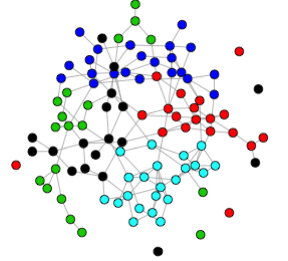
\includegraphics[scale = 0.5]{network.png}
		\end{center}
		\caption{An example of the initial state of a belief network \label{socnet}}
	\end{figure}
	
	\subsubsection*{Timing}
	
	The time periods $t$ are grouped in trading \emph{sequences}. In a given sequence, the potential payments associated with traded securities are all based on the temperature at the end of the sequence. For instance, the third trading sequence might start in period $t=300$ and end in period $t = 399$. In this case, a security traded in the third sequence pay 1 ECU if the temperature at $t=400$ falls into the range of temperatures covered by the security. 
	
	   At each time $t$, traders are assumed to know the past value of the temperature $T_{0:t}$ and the vector of past explanatory variables $Z_{0:t}$. In a sequence finishing at time $t^*$,  traders also have common knowledge of $Z_{t:t^*}$, the future values of explanatory variables up to $t^*$. However, at any $t$, traders do not know the value of any future temperatures. In particular, in a given sequence, traders do not know the value of $T_{t^*}$. Traders can only predict $T_{t^*}$ using their approximate model and their knowledge of $Z_{t:t^*}$. Notice that because $Z_{t:t^*}$ is common knowledge, in each period $t$ every trader $i$ with the same approximate model forms the same expectation 
	   \begin{align*}
	  \mu_{ti} \equiv E_t( T_{t^*} ~|~ T_{0:t}, Z_{t:t^*},  \text{ approximate model of } i \text { at } t).
	   \end{align*}
	   We assume that the probability density that trader $i$ associate with $T_{t^*} = \tilde{T}$ at any $t$ is
	   \begin{align*}
	   f_{it}(T) = \mu_{ti} + N(0, \sigma_T),
	   \end{align*}
	   
	   where $N$ stands for a normal distribution and $\sigma_T$ is a fixed number determined by the true variance of temperatures.       
	   
	    At each time $t$, traders
	\begin{itemize}
		\setlength\itemsep{0em}
		\item recalibrate their approximate model based on the new set of past data available at $t$,
		\item compute their belief-density for $T_{t^*}$ and use it to determine the expected value they attached to each security,
		\item and trade on the market based on their market strategy at $t$.
	\end{itemize}
	
	
	At $t^*$, when the sequence ends, there is only one security $s^*$ associated with a range of temperatures including the actual $T_{t^*}$. Thus,
	\begin{itemize}
			\setlength\itemsep{0em}
		\item traders receive 1 ECU per unit of $s^*$ they own, and
		\item  consider adapting their approximate model as described above.
	\end{itemize}
	
	\section{Implementation}
	\label{implem}
	The model is implemented in the \texttt{R} programming language,  using the \texttt{igraph} package to model the social network. Each trader in the model is a node of an \texttt{igraph} network. Because the model uses time-series data and  traders calibrate statistical models based on these data, \texttt{R}, primarily used for statistical computing, is particularly convenient. 
	
	 Traders calibrate their approximate models based on past-data using Pooled Ordinary Least Squares. This is questionable from a statistical point of view, but provides an approximation of the way traders may form their forecast on actual prediction markets. Because the model is in \texttt{R}, it is also very easy to change the estimation method or model to virtually any statistical model, and the effect of altering models may easily be studied in the future.
	
	 In each period $\tilde{t}$, our version of the CDA works as follows.
	
	\begin{enumerate}
			\setlength\itemsep{0em}
		\item Every trader $i$ choses at random a security $s_i^B$ she will try to buy.
		\item Every trader $i$ also chooses at random a security $s_i^S$ she will try to sell among the securities she owns a positive amount of (if any).
		\item Traders then decide of their selling $p_i^S$ and buying price $p_i^S$. They do so based on their believed-density of temperatures at the end of the sequence, and following the zero-intelligence rule described above.
		\item Traders go to the market one at the time, in a random order.
		\item When $i$ comes to the market, she place \emph{limit orders} in the order book. These orders  specify that $i$ is willing to buy $s_i^B$ at  any price below $p_i^B$, and to sell $s_i^S$ at any price above $p_i^S$.
		\item The market maker then tries to match $i$'s orders with some order which was put in the order book \emph{before} $i$ came to the market.
		\item If there are  outstanding sell offers for $s_i^B$ at price $p$ lower than $p_i^B$, then a trade is concluded. Trader $i$ buys one unit from the sellers who sells at the \emph{highest} price below $p_i^B$, and the sell and buy offers are removed from the order book.
		\item If there are  outstanding buy offers for $s_i^S$ at price $p$ higher than $p_i^S$, then a trade is concluded. Trader $i$ sells one unit to the buyer who buys at the \emph{highest} price above $p_i^S$, and the  sell and buy offers are removed from the order book.
		\item Whenever all traders have come to the market, any remaining outstanding offer is removed from the order book, and the trading period is concluded. 
	\end{enumerate} 
	
The model depends on the following parameters. 
\begin{description}
	\setlength\itemsep{0em}
	\item[Network parameters.]~
	\begin{description}
			\setlength\itemsep{0em}
		\item [\texttt{n.traders}:] the number of traders.
		\item [\texttt{n.edg} :] the number of edges in the social network. This number is fixed throughout the experiments.   
		\item [\texttt{seg} :] determines the initial degree of homophily in the network. The higher \texttt{seg}, the higher the initial homophily.\footnote{ When constructing the \texttt{n.edg} edges of the network, the probability that a link between two traders be formed depends on whether the traders share the same approximate model in the following way
			\begin{align*}
			\begin{cases}
			\frac{(1-\texttt{seg})}{\texttt{n.edg}},  &\text{if the traders have different approximate models}\\
			\frac{1}{\texttt{n.edg}},  & \text{otherwise}
			\end{cases}
			\end{align*}}
	\end{description}

\item[Market structure parameter.]~

		\begin{description}
			\setlength\itemsep{0em}
			\item [\texttt{market.complet}.] Determines market's completeness, i.e. the number of securities which can be traded. With more securities, the interval of temperatures corresponding to each security is smaller. Traders can then trade on more precise temperature intervals. Higher values of \texttt{market.complet} may, however, reduce the number of exchanges. Because traders pick the securities they buy and sell at random, the probability that a match between sellers and buyers is found is lower for higher values of \texttt{market.complet}.
		\end{description}
	 
\item[Behavioral parameters.]~

\begin{description}
	\setlength\itemsep{0em}
	\item [\texttt{risk.tak}.] Determines the distribution of risk taking behavior. The higher \texttt{risk.tak}, the more traders	will try to buy (resp. sell) lower (resp. higher) than their reservation price. Formally, at time $t$, trader $i$ picks her buying (resp. selling) prices randomly in the interval  $[\texttt{reserv}_{it}, \allowbreak \texttt{reserv}_{it}  * (1 - \texttt{risk.tak}_i)]$ (resp. $[\texttt{reserv}_{it}, \allowbreak \texttt{reserv}_{it} * (1  + \texttt{risk.tak}_i)]$), where $\texttt{reserv}_{it}$ is $i$'s reservation price at time $t$ for the security $i$ picked to buy (resp. sell).
	\item [\texttt{ideo}.]  Determines the degree of ``ideology" of traders. If \texttt{ideo} is high, traders will not
	 revise their approximate models easily, even when faced with
	 strong evidence that their neighbors are doing better than them.\footnote{ For each trader $i$ and each sequence, a parameter $d_{i}$ is drawn from $[0, \texttt{ideo}_i]$. The value of $d_{i}$ is the probability that $i$ adopts one of her neighbors' approximate model if this neighbor is doing better than $i$ at the end of the sequence (in monetary terms).}
\end{description}	 
	
	\item[Timing parameters.]~
	
	\begin{description}
			\setlength\itemsep{0em}
		\item [\texttt{burn.in}.] The number of burn-in periods in which no securities are traded (necessary to allow approximate models to be estimated in the first period).
		\item [\texttt{n.seq}.] Number of trading sequences.
		\item [\texttt{horizon}.] Number of trading periods in each trading sequence.
	\end{description}

\end{description}

	\section{Results}
	
	\label{results}
	
In this section, we present preliminary sensitivity analyses and exploratory results based on the above model.  In general, we will be interested in the fraction of traders who believe in the true model. For sensitivity analysis, the relevant outcome will be the difference between the fraction of traders who believe in the true model at the beginning of the experiment, and the fraction who believe in the true model at the end of all trading sequences. 

	\begin{figure*}
		\begin{center}
			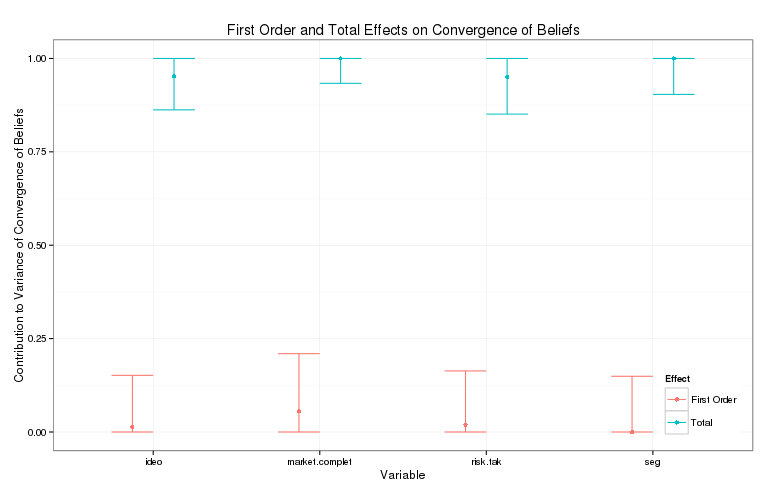
\includegraphics[scale = 0.5]{sobol_sa.png}
			\caption{ Effect of parameters on the difference between the initial and final fraction of traders who believe in the true model \label{nondirect}}
		\end{center}
	\end{figure*}

Before presenting these results, let us mention some important caveat. First, the model currently uses artificial data. The values of the explanatory variables are in not connected with the observed past values of greenhouse gas concentrations, GDP, etc. As a consequence, the results should be viewed as no more than a proof of concept, and no conclusions on actual {climate} prediction markets should be drawn from them. A second reason to be cautious about the following results is that they rely on varying only a handful of the model's parameters, namely
\begin{itemize}
	\item \texttt{ideo}, 
	\item \texttt{market.complet}, 
	\item \texttt{risk.tak}, and
	\item  \texttt{seg}.
\end{itemize}

Other parameters are fixed to the following values.

\begin{itemize}
	\item \texttt{n.traders} = 100,
	\item \texttt{n.edg} = 150,
	\item \texttt{burn.in} = 100,
	\item \texttt{n.seq} = 20, and
	\item \texttt{horizon} = 10.
\end{itemize}

We first present two sensitivity analyses for the four parameters above. Both sensitivity analyses are based on a Latin Hypercube Sampling of the four parameters, with uniform prior distributions. The support for the distributions are:

\begin{itemize}
	\item \texttt{ideo} : $(0,1)$
	\item \texttt{market.complet} : $ \{1,\dots,1000\}$,  
	\item \texttt{risk.tak}  : $(0,1)$, and
	\item  \texttt{seg} : $(0,1)$.
\end{itemize}
	
	The first analysis is similar to an ANOVA, and is based on  variance decomposition below \cite[Section 2.3.1]{Confalonieri2010}. Let the four varied parameters be denoted $x_i$ for $i =1,\dots,4$, and the difference between the final and the initial fraction of traders who believe in the true model be $Y$. Then we have
	\begin{align}
	\label{variance}
	V(Y) = \sum_{i=1}^4 \Big[  D_i + 
	\sum_{i \leq j \leq 4}^4 \big[ D_{ij} + \dots + 
	D_{1234} \big] \Big],
	\end{align}
	
	where $D_i = V(E[Y|x_i])$, $D_{ij} = V(E[Y|x_i,x_j]) - D_i - D_j$ and so on. Dividing both sides of \eqref{variance} by $V(Y)$ we obtain a normalized sum. The first terms of this normalized sum are
	\begin{align}
	S_i = \frac{V(E[Y|x_i])}{V(Y)},
	\end{align}
	which are called the first-order effects (of $i$). First-order effect $S_i$ represents the proportion of the variance which is explained by changes in $x_i$ once the effect of variations in the other $x_j$ ( $j\neq i$) has been accounted for. In Figure \ref{nondirect},  the value of $S_i$ is represented in red for the four parameters, together with their respective confidence intervals. One can see that none of the parameters' first-order effects is significant. 
	
	\begin{figure*}
		\begin{center}
			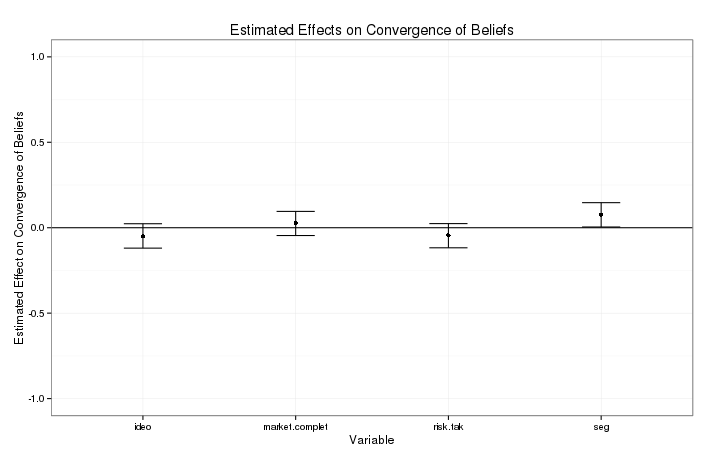
\includegraphics[scale = 0.5]{pc_sa.png}
			\caption{Partial rank correlation coefficients and confidence interval \label{prcc}}
		\end{center}
	\end{figure*}
	
	 Depicted in blue in Figure \ref{nondirect} are the total effects of the parameters. For each parameter $x_i$, the total effect corresponds to the sum of the net impacts of every possible combination of $x_i$ with other parameters. Formally, for each $x_i$ the blue dot and confidence interval in Figure \ref{nondirect} corresponds to
	 \begin{align}
	 \begin{split}
ST_i =  S_i  + \sum_{j\neq i}  S_{ij} + \dots +  S_{1234} 
 \end{split},
	 \end{align}
	 
	where  $S_{ij} = \sfrac{ V(E[Y|x_i,x_j]) - \allowbreak V(E[Y|x_i])- V(E[Y|x_j])}{V(Y)}$ and the other terms are defined similarly. Figure \ref{nondirect} indicates that most the effect of the parameters happens through interactions with other parameters.

	\begin{figure}
		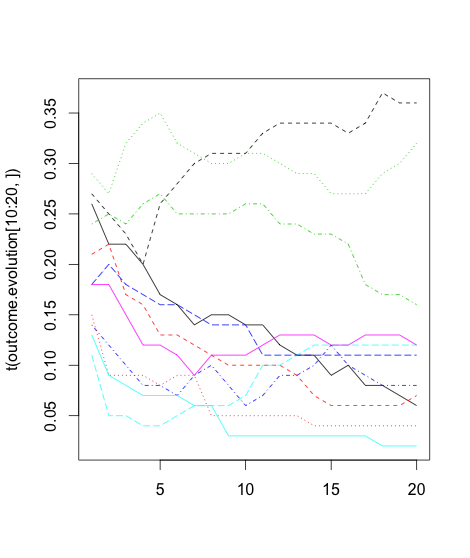
\includegraphics[scale = 0.4]{Rplot01.png}
		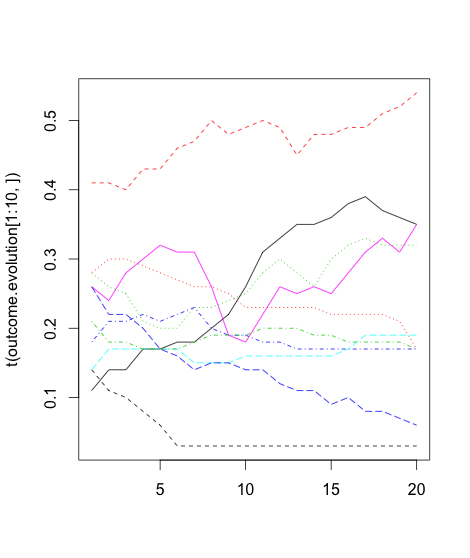
\includegraphics[scale = 0.4]{Rplot02.png}
		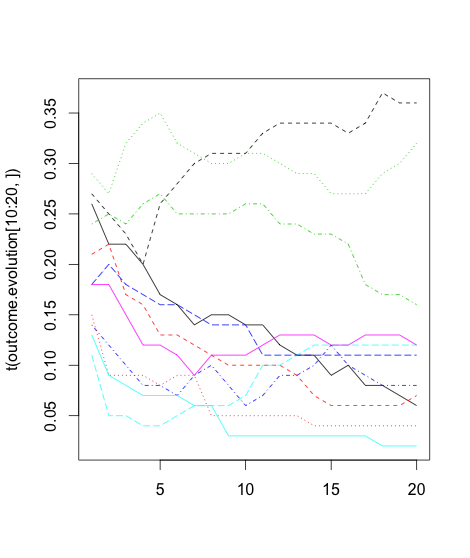
\includegraphics[scale = 0.4]{Rplot03.png}
		\caption{Evolution of the fraction of traders who believe in the true model (y-axis) as a function of the number of trading sequences (x-axis) for 30 random draws of the parameters.\label{example}}				
	\end{figure}


	The variance analysis does not provide information on the sign of the first-order effects. To investigate signed-effect, we turn to a second sensitivity analysis known as partial \emph{rank} correlation coefficient \citep{Marino2008}. Partial correlation computes the linear relationship between the part of the variation of $x_i$ and $Y$ that are linearly independent of other $x_j$  ($j \neq i$). First, we compute predicted value $\hat{x}_i$ and $\hat{Y}$ based on an OLS regression of $x_i$ and $Y$ on $x_j$  ($j\neq i$)
	\begin{align}
	\begin{split}
	\hat{x}_i = c^0_{OLS} + \sum_{j \neq i} c^j_{OLS} x_j,\\
	\hat{Y} = b^0_{OLS} + \sum_{j \neq i} b^j_{OLS} x_j.
	\end{split}
	\end{align}
	Then we compute the coefficient of correlation between $(x_i - \hat{x}_i)$ and $(\hat{Y} - \hat{Y})$. 
	
	The only difference with the partial correlation and partial \emph{rank} correlation (which we use here), is that the dependent variable $Y$ is first ranked-transformed in order to foster more uniform residuals.\footnote{That is every $Y_s$ in the data set is replace by a number $f(Y_s) \equiv |\{Y_r~|~ Y_s > Y_r\}|$, where $Y_r$ are the other observed values of $Y$ in the data set.} Such transformation preserves the sign of the correlation coefficient. However, because data are transformed, we loose the meaning of the coefficient's magnitude with respect to the original data. The partial rank correlation coefficients are reported in Figure \ref{prcc}. 
	
	 It is surprising that the net effect of \texttt{seg} on $Y$ is positive. This suggests that a higher initial belief-homophily in the network increases (or reduces the decrease in) the adoption of the true model. Intuitively, traders endowed with the correct explanatory model should be better at predicting climate outcomes. Therefore, if they are connected to traders with different approximate models, one could expect that these other traders will eventually adopt the true model. If that were true, the more traders endowed with the true model are disseminated across the network (i.e. the smaller \texttt{seg}) the better the result should be in terms of adoptions of the true model. The results  in Figure \ref{prcc} indicates that, if at all present, this kind of dynamics are not sufficient to explain changes in the adoption of the true model.
	
	Exploratory investigations also cast a doubt on the ability of the modeled prediction market to foster convergence to the true model. Figure \ref{example} contains plots for the evolution through trading sequences of the fraction of traders who believe in the true model. Each line corresponds to a different random value for the four parameters. The figure show a wide variety of dynamics and indicate that under many parameter configurations, the fraction of traders who believe in the true model significantly reduces (sometimes almost completely).
	
	Finally, it appears that the current version of the model is too random. Figure \ref{random} represents the evolution of $Y$ for 10 different runs of the model \emph{using the same value for the parameters}, namely 
	
	\begin{itemize}
		\item \texttt{ideo} = 0.5,
		\item \texttt{market.complet} = 100,
		\item \texttt{risk.tak} and = 0.02, and
		\item  \texttt{seg} = 0.5.
	\end{itemize}
	
	As can be seen from the figure, a lot of randomness is built into the model independently of changes in the parameters. For instance, notice that the initial fraction of agents who believe in the true models varies from one run of the model to the other.  The probability that a trader starts with the true model is fixed at $\sfrac{1}{5}$. But only 100 traders are assigned an initial approximate models which explains such variability. Other randomness built into the model includes the distribution of the risk and ideology parameters $\texttt{risk.tak}_i$ and $\texttt{ideo}_i$.\footnote{Currently, $\texttt{risk.tak}_i$ is drawn at random from $[0, \texttt{risk.tak}]$. Thus, increasing \texttt{risk.tak} increases the chance that traders have higher $\texttt{risk.tak}_i$, but there is a significant amount of randomness in the assignment of the $\texttt{risk.tak}_i$. The same is true for $\texttt{ideo}_i$.} This might partly explain why we do not get clearer results in the sensitivity analysis.
	
	\section{Conclusion}
	
	In this report, we described a minimal ABM of a climate prediction market in which traders adapt their belief of the climate based on the monetary performance of their neighboring traders in a social network. The market mechanism is a variant of the famous continuous double-auction, and traders are risk-neutral expected utility maximizers who behave on the market as zero-intelligence agents \citep{Gode1993}.
		\section{Related Work}
	Future developments involve :
	
	\begin{itemize}
		\item Reducing the randomness built in the model and simplify the model in order to obtain clearer results. One way of simplifying the model would be to reduce the number of approximate models (e.g. anthropogenic climate change is a myth vs. anthropogenic climate change is true).
		\item Implementing a second market rule (LMSR, \cite{Hanson2012}).
		\item Using actual time-series data for the temperature and the explanatory variables. At this stage, the data used in the model are randomly generated time series with no connection to actual temperatures, or to observed values of the explanatory variables.
		\item Varying more parameters. In particular, changes in timing parameters should be studied in order to tackle the issue of optimal timing in climate prediction markets.
		\item Studying the model under different assumption about the true model in order to check whether climate prediction markets are an apartisan proposal.
	\end{itemize}
	
	\begin{figure}
		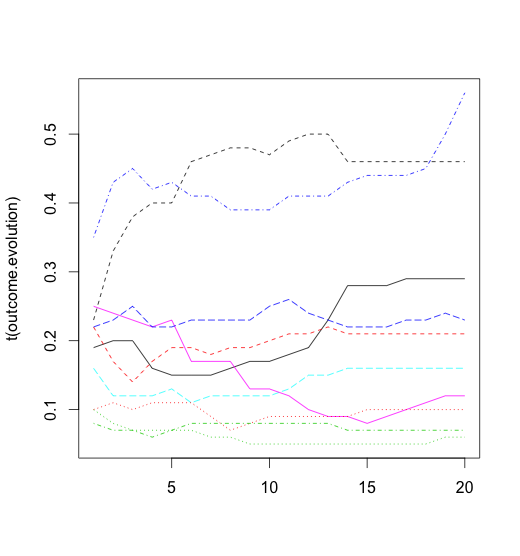
\includegraphics[scale = 0.4]{random.png}
		\caption{Evolution of the fraction of traders who believe in the true model (y-axis) as a function of the number of trading sequences (x-axis) for 10 different run of the model with \emph{fixed} values of the parameters ( \texttt{ideo} = 0.5,
			 \texttt{market.complet} = 100,
			 \texttt{risk.tak} and = 0.02, and
			  \texttt{seg} = 0.5.). \label{random}}
	\end{figure}
	
	\bibliography{library}
	\bibliographystyle{apalike}
	
\end{document}
